In this chapter, we focus on \emph{Pacman} as learning environment and on our collection of agent programs based on deep Q-learning.

The project itself consists of a light framework for training, running and evaluating RL agents.
Our framework is compatible with various other environments, as long as they respect the interface provided by OpenAI Gym.
The feature set includes automatic checkpoints, cloud-friendly deployment and a performance analysis toolkit.

In Section \ref{section:modelling-the-problem}, we justify why we choose to study the game of \emph{Pacman} and formalize the specifications of it as a learning environment.

In Section \ref{section:approach-algorithms}, we introduce some of the algorithms built into our collection of autonomous agents.
The main method is vanilla DQN, which was covered previously in Section \ref{section:dqn}.
However, in this section, we present two important improvements over it -- Double DQN and Prioritized Experience Replay.

In Section \ref{section:implementation}, we take a look at each subcomponent of an individual agent program and map each one to notions from our previous chapter.
Each agent has its own module and inherits a specific structure from a prototype.

In Section \ref{section:technologies}, we present a rundown of our technology stack, whose core is the Python programming language. The framework is built on the PyTorch machine learning library but makes use of many other ML and data science libraries.

We wrap up this chapter with Section \ref{section:user-manual} which consists of a short instruction manual for users to start local or remote training sessions, use the provided performance measurement tools and extend the existing collection of agents.

\clearpage

\section{Modelling the Problem} \label{section:modelling-the-problem}
The problem we solve in this thesis is three-fold.
Firstly, we specify a variant of a task environment for \emph{Pac-Man}, defining goals and rewards to view it through the lens of reinforcement learning.
Secondly, we train agents to ``solve’’ that environment, i.e. explore and learn to take optimal decisions to achieve the established goals.
And lastly, we compare agents based on their how close they were to their goals, what their mean reward was and how stable was their learning process.

\textbf{\textit{Pac-Man}} is a classic video game developed by Toru Iwatani and published by Namco Ltd. in 1980 \cite{pacman-in-academia}.
The game was originally released as an arcade game and it quickly became the most commercially sucessful arcade game ever created.
The original hit gave rise to a series of ``licensed clones'', which targeted a number of popular platforms, such as the Atari 2600, the Nintendo Entertainment System (NES), the Nintendo GameBoy, etc.
Besides its commercial success, \emph{Pac-Man} has been an appealing object of study for academia, across a number of fields, ranging from psychology to mathematics and computational intelligence \cite{pacman-in-academia}.

\begin{figure}[h]
    \centering
    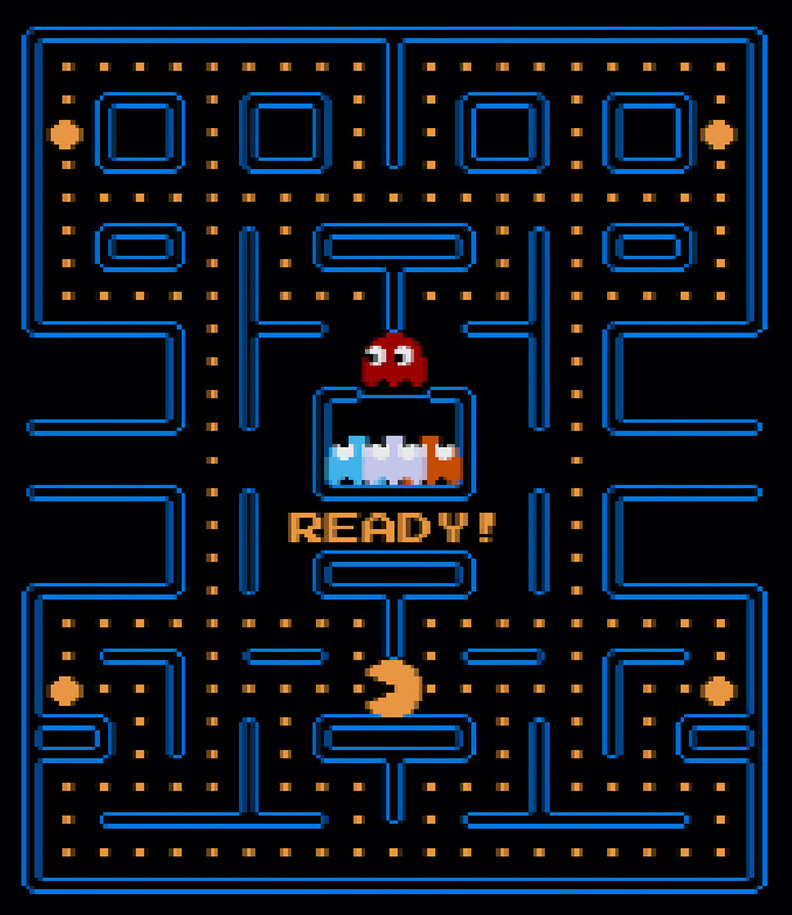
\includegraphics[width=0.4\textwidth]{nes-pac-man.jpg}
    \caption{Screen capture of the starting configuration from Nintendo's NES variant of the game.}
    \label{fig:pac-man-screen}
\end{figure}

The game's mechanics are intuitive but engaging enough to be fun.
It allows simple four-directional movement.
The player is represented as a yellow character with a distinctive circular shape (with a ``missing slice''\footnotemark{} representing its mouth).
\footnotetext{Iwatani's stated inspiration for Pac-Man's design was a pizza with a missing slice. \cite{pacman-gameinformer}}
The board is a bidimensional maze, featuring tunnels which loop around each other, i.e. entering a tunnel on one side will transport the player out through the opposite side of the board.
\textbf{Pellets} (or \emph{dots}) are placed at almost every position, and the goal of every level is to collect all pellets.
Most renditions of the game feature four \textbf{ghosts} (faithful to the original), which will chase the player around the board.
Collisioning with any of the ghosts results in losing a life and being repositioned to the start (without losing progress on dots).
The ghosts have different ``personalities'' -- each of them has a different approach for chasing Pac-Man.
There are special power pellets in each of the four corners (seen in Figure \ref{fig:pac-man-screen}).
\textbf{Power pellets} grant Pac-Man temporary immunity from ghosts and changes the power dynamic in the game for a short time: the ghosts enter \textbf{``scared'' mode} and reverse their direction to run away.
In this mode, the player gets an increasing score for every ghost it eats.

\emph{Pac-Man} can be defined as a 2D gridworld environment, where exploration is necessary to reach the goal.
This class of task environments is common throughout RL literature and has some common properties:
\begin{itemize}
    \item they have discrete bidimensional representation;
    \item an agent has a finite set of options at every time step.
\end{itemize}

\textbf{Gridwords} are used in literature to clearly define and \textbf{isolate} agent goals.
A simplistic environment with a clear task is also beneficial for agent learning due to its low degree of environmental noise -- it does not ``distract'' the agent.
The ease of customizability of the rules inside a gridworld allows creating interesting strategy games to test agents’ decision-making capabilities.
New non-trivial grid-based environments are an area of open research -- for example, the \emph{Pommerman} benchmark \cite{pommerman-paper} has been formulated as a novel interesting multi-agent problem which does not yet have an optimal solution.

\emph{Pac-Man} has a few advantages which make it interesting to study from a RL perspective.

First of all, it provides a \textbf{shaped reward} built-into the game mechanics.
In reinforcement learning, a \textbf{sparse reward} is a large reward which is delayed for a relatively large number of steps.
A sparse reward would be, for example, if we would only reward the agent at the end of the game.
Shaped rewards, in contrast, equate with providing gradual feedback to the agent.
This can improve learning and lead to better outcomes earlier in training, as good behaviours become immediately obvious to the agent.

In \emph{Pac-Man}, the pellets, placed uniformly over the board, provide a shaped reward which directly reflects the goal of the game, i.e. to eat all pellets on a board without getting caught.
Moreover, they \textbf{incentivize exploration} as the reward is higher in places the agent has not visited before.

Second of all, \emph{Pac-Man} requires the agent to develop non-trivial strategies.
The game requires balancing two equally important subgoals: fully covering the game board to consume every available pellet, and running away from the chasing ghosts.
This gives rise to complex and potentially problematic situations for the player, which require \textbf{planning}.
This raises an interesting question regarding the potential of existing algorithms to learn \textbf{long-term strategies} similar in performance to human players.

The \textbf{reward function} we use in this thesis for our \emph{Pac-Man} environment is a combination of a few properties of the environment state.
The most important component is the \textbf{score}.
Score changes will determine a proportional reward for the agent.
Significant score increases are provided by eating pellets but a more interesting mechanic is eating ghosts when the player is invincible.
Each ghost eaten will provide a higher reward, thus conditioning the agent to chain as many ``kills'' as possible.
Typical of arcade games, the mechanics are built such that the score can \emph{only increase} over time.
This creates a necessity to \emph{counterbalance} by finding opportunities for \textbf{punishment}.
We choose to strongly penalize the the agent for losing a life.
There are other possible candidates for ``punishment'' events, but we consider ``death on ghost contact'' to be the most important for capturing the goal of the game.

\section{Algorithms} \label{section:approach-algorithms}
In this section, we present the main algorithms powering the autonomous agents evaluated in this thesis. In our collection, \textbf{vanilla DQN} serves both as a stand-alone implementation, as well as a fundamental building block of more advanced algorithms.
The original DQN, however, is already covered by Section \ref{section:dqn} of our theory chapter and we will omit it here for conciseness.
Instead, this section deals with \textbf{double DQN} and \textbf{prioritized experience replay (PER)}, both of which address shortcomings of the original algorithm.

\subsection{Double Q-learning}
Double DQN \cite{ddqn-paper} is an algorithm in the deep Q-learning family, discovered and published by DeepMind researcher Hado van Hasselt along with several other colleagues.
The study determines that general Q-learning (and, by extension, deep Q-learning) suffers from a problem known as a \textbf{maximization bias} and adapts the original algorithm to account for this and counteract the bias.

Stated simply, a \textbf{maximization bias} is an implicit preference of the algorithm to overestimate values, despite divergence from the true value.
Some control algorithms, such as Q-learning, fundamentally depend on using the maximum over estimated values as an estimate for the maximum value \cite{rlai}.
This leads to situations where noisy reward signals, prevalent in real-world environments, can significantly destabilize learning and slow down training progress.

Hasselt proposes \emph{double learning} to counteract this bias.
This requires two independent approximators of the action-value function -- we will denote them $Q_1$ and $Q_2$.
At every step, the approximators are \emph{intermittently} used either to pick an action or to estimate its value.
The paper proves that this decoupling is sufficient to accomplish an unbiased estimation.
Which function serves which role can be chosen uniformly at random at every learning step at practically no cost.
Equation \ref{eqn:double-learning-rule} states the double learning \textbf{update rule}, considering the situation in which $Q_1$ picks the action (and is updated) while $Q_2$ gives the estimate which we bootstrap from.

\begin{equation} \label{eqn:double-learning-rule}
\begin{aligned}
Q_1(S_t, A_t) & \leftarrow Q_1(S_t, A_t) \\
    & + \alpha [ R_{t+1} + \gamma Q_2(S_{t+1}, \argmax_{a \in A} Q_1(S_{t+1}, a)) - Q_1(S_t, A_t)]
\end{aligned}
\end{equation}

A drawback of the double learning algorithm is that it requires double the amount of memory of the original. 
Despite this, it still performs one update per step, so the running time is equivalent to that of its predecessor.
% to steal more content space, include and explain the example from RLAI

\subsection{Prioritized Experience Replay (PER)}
\textbf{Prioritized experience replay} (often shortened as \emph{PER}) is an extension of deep Q-learning, also developed by a team at DeepMind, led by Tom Schaul \cite{per-paper}.
The paper focuses on improving experience replay from classic DQN.

Recall from Section \ref{section:dqn} the principle of \textbf{experience replay}, which consists of storing all transitions the agent experiences in order to revisit them later during training.
Reusing experiences over multiple update steps reduces the number of samples required for learning.
The original approach suggests that the experiences are revisited by sampling them uniformly at random from the replay memory.
This has the important role of \emph{decoupling} experiences -- which in the case of successive video game frames, are by nature highly correlated -- to avoid introducing \emph{high variance} into the system (which can cause overfitting).

The foundational hypothesis of the paper at \cite{per-paper} is that some transitions have higher ``teaching’’ potential than others.
The \emph{prioritization} mentioned in the title refers to finding an ordering over experiences which properly reflects this potential.
The authors chose \emph{absolute TD-error} as a good approximation for utility in learning -- for several reasons.
Firstly, since larger errors suggests that a prediction is further from the agent’s current expectations, minimizing larger error would naturally improve 
This supposition has intuitive appeal because \textbf{humans} likewise learn proportionally more from experiences that contradict their existing beliefs the most.
Additionally, TD-error is already computed as part of the normal update cycle in DQN so extending the implementation to PER does not require significant overhaul of the algorithm.

The paper develops two separate models for prioritizing experience based on error.
Each model specifies how priorities are computed and stored.

\textbf{Rank-based prioritization} involves keeping track of the rank each transition occupies.
Each transition would thus have an assigned priority of $p = 1 / rank$.
This requires an additional data structure, capable of online sorting, such as a heap, as some ranks will change at every update step.

Since the replay memory can potentially store millions of transitions, \textbf{optimization} is necessary to prevent severely hindering performance.
Changing every rank at every update step is impractical and would outweigh the benefits of prioritization.
In order to mitigate this, the authors propose to only re-evaluate the ranks of transitions in the sampled mini-batch.
This \textbf{``lazy’’ approach} retains its desirable properties of learning more efficiently than DQN while not adding an insane amount of computation.

\textbf{Proportional prioritization} simply assigns a priority equal to the absolute TD-error plus an $\epsilon$: $p_{i} = |\delta_{i}| + \epsilon$.
The $\epsilon$ (which should not be confused with our exploration coefficient in $\epsilon$-greedy) is an offset keeping all priorities above $0$.

The second part of the algorithm is common to both models and consists of actually assigning probabilities based on priority and building the distribution over the transitions. The formula in (\ref{eqn:per-probability}) gives an outline of the method.

\begin{equation} \label{eqn:per-probability}
    P(i) =  \left( \frac{p_i}{\sum_{k}{p_{k}}} \right)^\alpha
\end{equation}

The $\alpha$ parameter in this equation represents the degree of prioritization, i.e. a higher $\alpha$ will determine a larger difference between the probabilities of any two priorities.

To sample according to the obtained priority, a sum tree is used.
A \textbf{sum tree} is a type of segment tree -- a tree data structure which stores statistics (minimum, maximum, sum etc.) of its leaf nodes (which also represent an array).
The structure is designed to compute interval queries, such as the sum between indices $x$ an $y$, in $\mathcal{O}(\log{n})$, while also allowing fast updates to the underlying data.

\section{Implementation} \label{section:implementation}
% show a conceptual overview of each high-level moving part
% and how they communicate
% Trainer class as an entry point
% show the class diagram and explain more low-level details}

\section{Technologies} \label{section:technologies}
% PyTorch, Google Cloud Compute, OpenAI Gym, Jupyter Lab
% In the future, TensorBoard

\section{User Manual} \label{section:user-manual}
% Commands for training, running, deploying, flags and configuration variables